\documentclass{report}
\usepackage[utf8]{inputenc}
\title{DeSem}
\author{Rémy Macherel}
\date{\today}
\usepackage[utf8]{inputenc}
\usepackage[T1]{fontenc}
\usepackage[english]{babel}
\usepackage{hyperref}
\hypersetup{
    colorlinks=true,
    linkcolor=blue,
    filecolor=blue,      
    urlcolor=blue,
    pdftitle={DeSEm project report},
    pdfpagemode=FullScreen,
    }
\usepackage{lmodern}
\usepackage{url}
\usepackage{wrapfig}
\usepackage{graphicx,subfigure}
\usepackage{textcomp}
\usepackage{float}
\usepackage{lastpage}
\usepackage{wrapfig}
\usepackage[top=3cm, bottom=3.5cm, left=3cm, right=3cm]{geometry}
\usepackage{fancyhdr}
\usepackage{lastpage}
% \usepackage[dvipsnames]{xcolor}
\usepackage{titlesec}
\usepackage{setspace}
%\usepackage{minted}
\usepackage{multirow}
\usepackage[export]{adjustbox}
\usepackage{subfigure}
\usepackage{titlesec}
\usepackage{setspace}
\usepackage{tikz}
\usepackage{tabto}
\usepackage{ragged2e}
\usepackage{pdfpages}
\usepackage[sorting = none]{biblatex}
\usepackage{csquotes}
\usepackage{enumitem}
\usepackage{caption}
\usepackage{amsmath}



\setcounter{tocdepth}{3}
\setcounter{secnumdepth}{3}
\pagestyle{fancy}
\fancypagestyle{plain}{}
\setlength{\headheight}{55pt}
\renewcommand\headrulewidth{1pt}
\fancyhead[L]{
\includegraphics[scale = 0.2]{./Images/Base/LogoHESSO.png}}
\fancyhead[R]{
\includegraphics[scale = 0.3]{./Images/Base/LogoMSE.png}}
\fancyhead[C]{DeSenet Laboratory}
\fancyfoot[L]{Page \thepage ~sur \pageref{LastPage}}
\fancyfoot[C]{Rémy Macherel}
% \fancyfoot[R]{Yverdon-les-Bains, le \today}
\titleformat{\chapter}[hang]
  {\normalfont\LARGE\bfseries}
  {\thechapter.}{1em}{\LARGE}
  \titlespacing*{\chapter}{0pt}{10pt}{10pt}


\makeatletter
\let\mytitle\@title
\let\myauthor\@author
\let\mydate\@date
\makeatother


\begin{document}

\begin{titlepage}
% \hspace{0pt}
% \vfill
 \line(1,0){420}
	\begin{center}
	\huge{\textbf{\mytitle}} \\
	\huge{DeSenet laboratory report}\\
	\LARGE{\myauthor} \\
	\LARGE{\mydate}
 \line(1,0){420}
 \end{center}
\textbf{\underline{Authors :}} \hfill \textbf{\underline{Teacher : }}\newline
Macherel Rémy \hfill Rieder Medard\newline
\hfill Sterren Thomas
\end{titlepage}

\renewcommand{\contentsname}{Table des matières}
\setcounter{tocdepth}{4}
\tableofcontents

\chapter{Introduction}
Dans le cadre du cours MA-DeSem, il nous a été demandé de réaliser le protocole DeseNET sur un système de type STM32 Nucleo. Les spécifications du protocole de communication ont été fournies pour ce travail.\newline
La structure de base du projet fût fournie et nous avons du apporter les modifications nécessaires au bon fonctionnement du protocole.
\chapter{Modifications du code}
\begin{figure}[H]
    \centering
    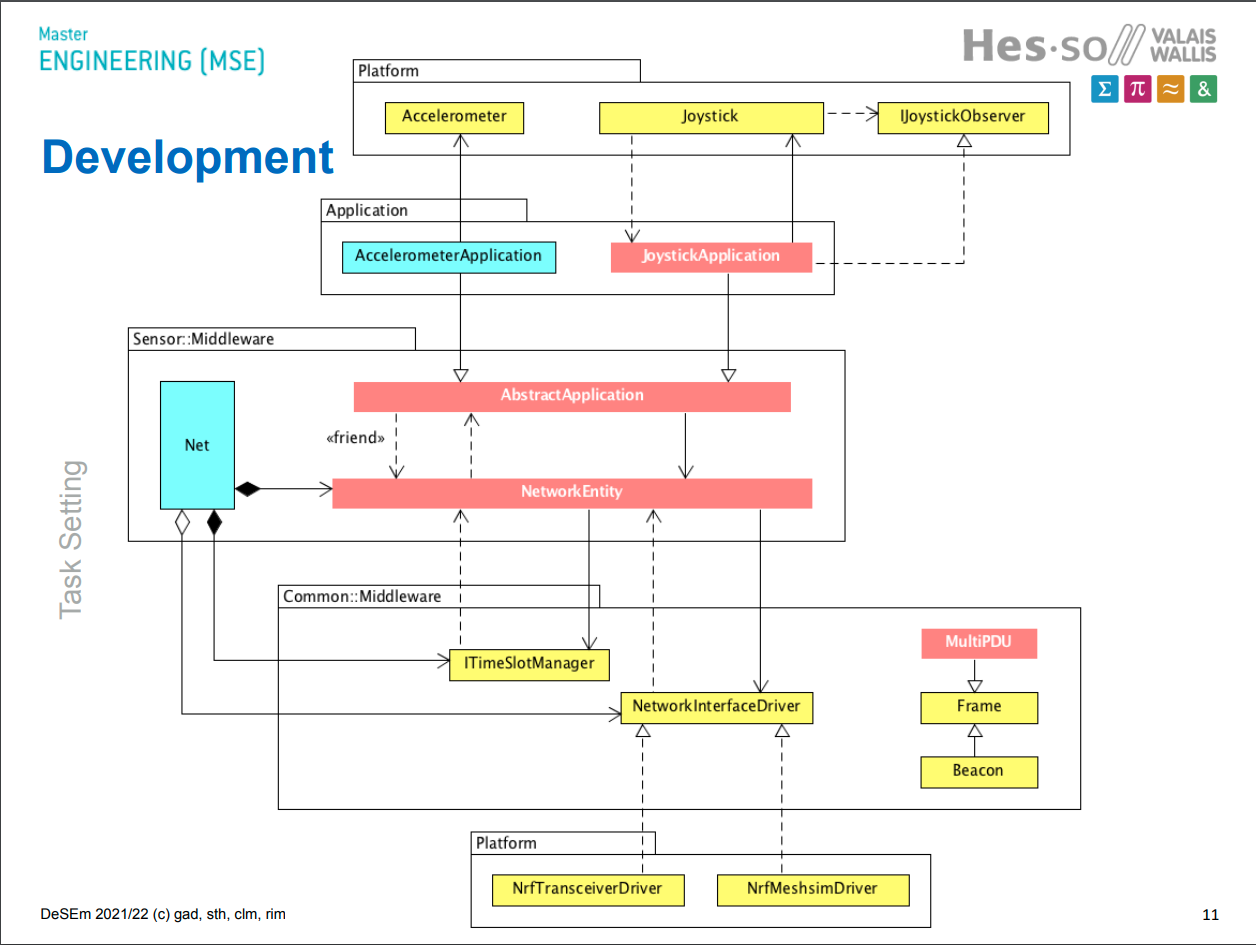
\includegraphics[width= 0.8\textwidth]{Images/ClassesToImplement.png}
    \caption{Aperçu des modifications à apporter}
    \label{fig:ClassesToModify}
\end{figure}
La figure suivante nous a été présentée afin d'illustrer les classes que nous devions compléter/créer. Les classes à créer sont les suivantes :
\begin{enumerate}
\item JoystickApplication (.h et .cpp)
\item MPDU (.h et .cpp)
\end{enumerate}
Alors que les classes à compléter sont :
\begin{enumerate}
\item AbstractApplication (.h et .cpp)
\item NetworkEntity (.h et .cpp)
\end{enumerate}
D'autres fichiers ont cependant également été modifiés comme par exemple Factory.cpp afin d'y ajouter l'initialisation du Joystick ainsi que le setObserver().\newline

\chapter{Classes implémentées}
\section{MPDU}
\begin{figure}[H]
    \centering
    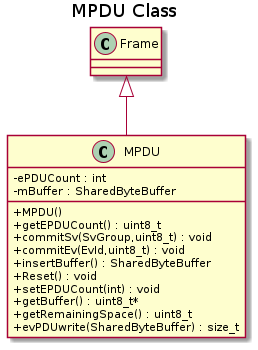
\includegraphics[width= 0.3\textwidth]{Images/MPDU.png}
    \caption{Diagramme de la classe MPDU}
    \label{fig:MPDUDiagram}
\end{figure}
Comme on peut le voir sur cette figure, la classe MPDU hérite de la classe \textit{Frame}. Ceci va permettre de réutiliser de nombreuses fonctions déjà implémentées dans celle-ci. 
\subsection{Méthodes implémentées}
\subsubsection{MPDU()}
Cette méthode est le constructeur, elle permet d'initialiser également la classe parent \textit{Frame} en lui passant en paramètre la variable \textit{Mtu} (égale à 37) qui représente la taille maximale d'une Frame.
\subsubsection{getEPDUCount()}
Cette méthode permet d'obtenir le nombre de EPDU qui sont actuellement dans la Frame. La valeur de ce compte est également écrite dans la Frame en question.
\subsubsection{commitSv(SvGroup,uint8\_t)}
Cette méthode permet de finaliser l'écriture d'une \textit{SampleValue (Sv)} en ajoutant dans la Frame le header de celle-ci. Le header est composé de trois champs :
\begin{itemize}
\item count : la taille en bytes de la valeur
\item svGroupOrEvId : Le numéro du groupe auxquel l'application s'est inscrite ou l'Id de l'évènement (pour les valeurs event, voir plus tard)
\item type : 0 pour sampleValue et 1 pour event 
\end{itemize}
Les paramètres de cette fonction sont l'identifiant de groupe (type SvGroup) et le byteCount (type uint8\_t).
\subsubsection{commitEv(EvId,uint8\_t)}
Comme la précédente méthode, celle-ci se charge de finaliser l'écriture d'un event dans la trame. Son fonctionnement est identique hormis qu'elle inscrira dans le champ type du header la valeur 1. Les paramètres sont l'identifiant de l'évènement ainsi que le byteCount.
\subsubsection{insertBuffer()}
Retourne un proxy du buffer principal (issu de Frame) qui permet d'inscrire des valeurs dans le buffer du MPDU. Le début du buffer renvoyé par cette fonction varie en fonction du contenu du buffer du MPDU.
\subsubsection{reset()}
Cette méthode sert à réinitialiser le MPDU afin qu'il soit à nouveau prêt à être réécrit pour de nouvelles données.
\subsubsection{setEPDUCount()}
Cette méthode sert à écrire au bon endroit dans le buffer le compte actuel de EPDU contenus dans le buffer.
\subsubsection{getBuffer()}
Cette méthode fut utilisée dans networkentity au moment de transmettre le MPDU. Elle ne fait qu'appeler la méthode buffer() de la classe Frame mais celle-ci étant déclarée protected, elle ne peut être appelée depuis l'extérieur de la classe MPDU. La méthode getBuffer() sert donc à contourner ceci.
\subsubsection{getRemainingSpace()}
Cette méthode est utilisée lors de l'écriture des EvPDU dans le networkentity afin de connaître l'espace disponible restant dans le buffer du MPDU.
\subsubsection{evPDUWrite(SharedByteBuffer}
Utilisée afin d'écrire les données d'un evPDU (ici une position du Joystick) dans le buffer du MPDU. Les evPDU étant basés sur un évènement et donc pas inscrits dans le publishArray, j'ai créé cette méthode afin d'inscrire la valeur de l'event dans le buffer.

\subsection{Séquence générique d'écriture d'un MPDU}
\begin{figure}[H]
    \centering
    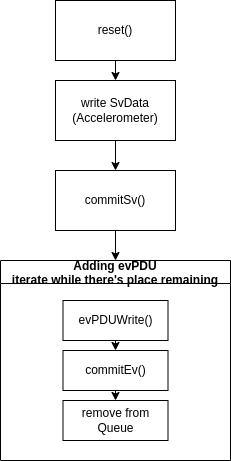
\includegraphics[width= 0.3\textwidth]{Images/MPDUWrite.png}
    \caption{Séquence d'écriture du MPDU}
    \label{fig:MPDUSequence}
\end{figure}
Ci dessus sont les étapes suivies lors de l'écriture d'un MPDU, ces étapes utilisent les méthodes précédemment décrites de la classe MPDU et sont réalisées dans la méthode \textit{onReceive()} de la classe \textit{NetworkEntity}. 

\subsection{svPDU}
Un svPDU représente une \textit{Sample Value}, c'est-à-dire une valeur mesurée par un capteur (dans notre cas l'accéléromètre). Afin d'écrire la valeur dans le MPDU (étape 2 de la séquence de la figure \ref{fig:MPDUSequence}), on vérifie que le beacon réceptionné demande bien les valeurs du groupe dans lequel notre mesure est effectuée. Si le beacon demande cette mesure, on va appeler la méthode \textit{svPublishIndication} de l'application contenue dans le groupe souhaité (ici l'accéléromètre) en lui passant en paramètres un proxy du buffer du MPDU dans lequel cette méthode se chargera d'inscrire ses valeurs (exemple pour notre cas : la méthode \textit{svPublishIndication} dans le fichier \textit{AccelerometerApplication.cpp}). La méthode \textit{commitSv()} permettra ensuite de finaliser l'écriture de cette sample value.
\subsection{evPDU}
Le deuxième type de valeurs reçues dans ce projet sont les valeurs reçues par évènement. Ces valeurs sont dans notre cas des positions de click sur le Joystick. Pour l'écriture de ces valeurs, le protocole prévoit d'ajouter autant de evPDU qu'il reste de place dans le buffer du MPDU. Lorsque soit la queue d'évènements est vide ou que le MPDU n'a plus de place, le MPDU est prêt à être transmit. Note : S'il reste des évènements dans la queue, celle-ci sera vidée lorsque le MPDU est plein, ceci peut engendrer la perte de certains évènements mais permet également de ne pas "polluer" les prochains timeSlots et ainsi retarder la réception de certains évènements.
\subsection{Transmission du MPDU}
Le projet est défini sur un système de Time Slots, c'est-à-dire que chaque station a sa période durant laquelle elle peut transmettre des données au Gateway. Afin de transmettre le MPDU, on utilisera la méthode \textit{onTimeSlotSignal()} de \textit{NetworkEntity}. Dans cette méthode on vérifie que le signal du timeslot correspond bien à un start de notre timeSlot (OWN\_SLOT\_START) puis on appelle 
transceiver().transmit(responseMPDU.getBuffer(),responseMPDU.length()) qui va transmettre au Gateway le MPDU construit selon les étapes ci-dessus.
\section{JoystickApplication}
\begin{figure}[H]
    \centering
    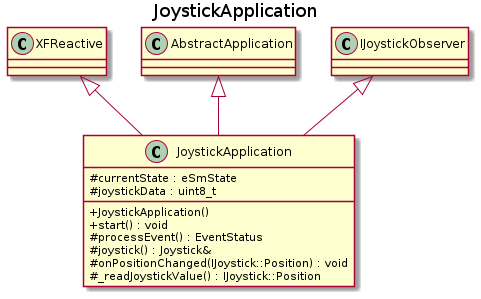
\includegraphics[width= 0.5\textwidth]{Images/JoystickApp.png}
    \caption{JoystickApplication UML Diagram}
    \label{fig:JoystickAppUML}
\end{figure}
Cette classe fut construite en se basant sur la classe \textit{AccelerometerApplication}, et hérite de AbstractApplication (classe abstraite de base pour les applications), de IJoystickObserver (afin de pouvoir utiliser la méthode \textit{onPositionChanged()}), et de XFReactive (utilisé pour la machine d'état).
\subsection{Propriétés}
Les propriétés de cette classe sont \textit{currentState} qui contient l'étape actuelle de la machine d'état de l'application et \textit{joystickData} qui contient la valeur de la position du joystick.
\subsection{Méthodes implémentées}
\subsubsection{JoystickApplication()}
Le constructeur de cette classe permet d'initialiser ses propriétés. Il permet également de définir l'état initial de la machine.
\subsubsection{start()}
Cette méthode permet d'appeler la méthode \textit{startBehavior()} héritée de XFReactive qui permet de démarrer la machine d'état via XFReactive.
\subsubsection{processEvent()}
Cette méthode est utilisée afin d'implémenter la machine d'état (qui sera décrite plus bas) et de traîter les évènements.
\subsubsection{joystick()}
Cette méthode sert à récupérer le singleton correspondant au Joystick() depuis la Factory.
\subsubsection{onPositionChanged(IJoystick::Position)}
Cette méthode héritée IJoystick permet de générer un évènement XFReactive de type \textit{POSITION\_CHANGED\_EVENT} (voir explications de la machine d'état).
\subsubsection{\_readJoystickValue()}
Cette méthode utilise l'instance de Joystick afin de récupérer sa position actuelle.
\subsection{Machine d'état}
\begin{figure}[H]
    \centering
    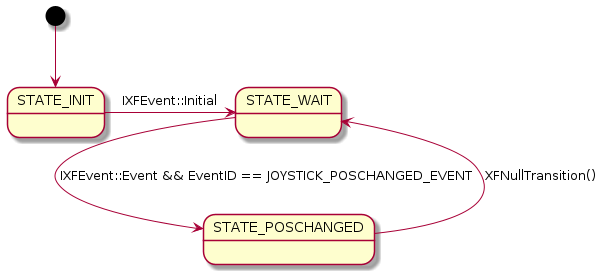
\includegraphics[width= 0.7\textwidth]{Images/SMDiagram.png}
    \caption{JoystickApplication machine d'état}
    \label{fig:SMJoystickApp}
\end{figure}
La machine d'état implémentée pour la classe \textit{JoystickApplication} est celle présentée dans la figure \ref{fig:SMJoystickApp}, lors de la réception d'un évènement de type \textit{IXFEvent::Initial}, on passe dans l'état wait, puis, à la réception d'un évènement ayant comme Id JOYSTICK\_POSCHANGED\_EVENT, on passe dans l'état STATE\_POSCHANGED. La machine d'état a été implémentée selon le principe du double switch vu en cours.
\chapter{Diagramme de séquence de l'application}
\begin{figure}[H]
    \centering
    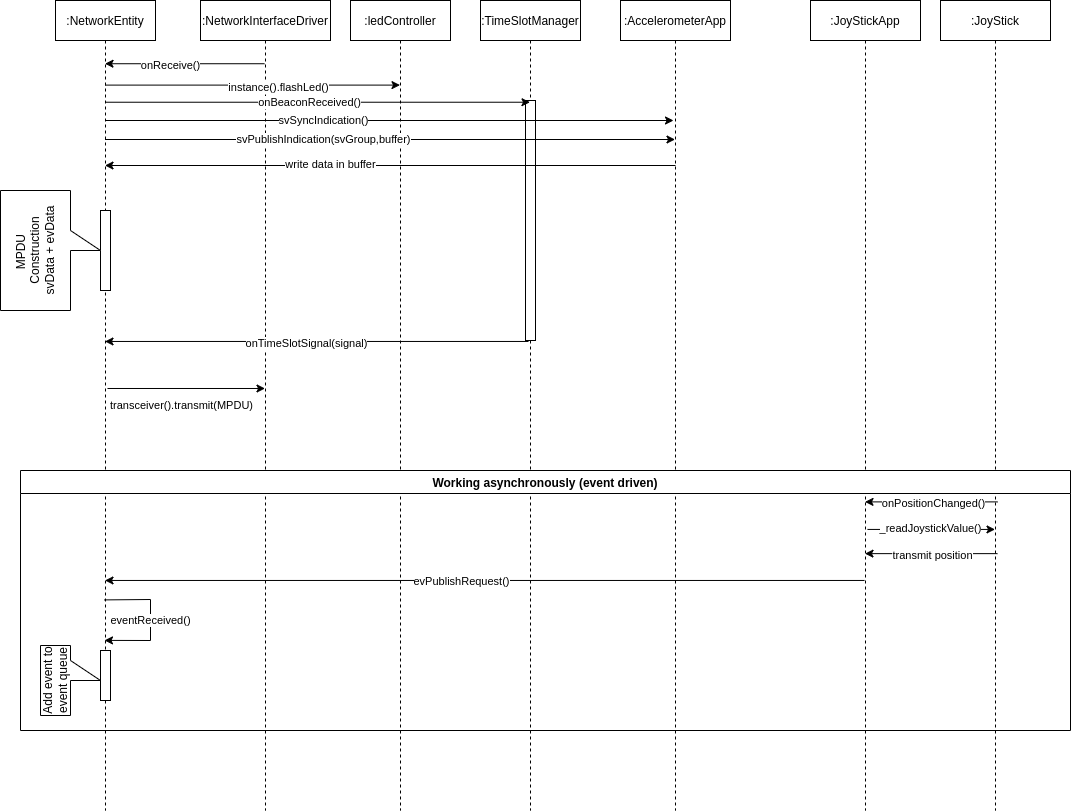
\includegraphics[width= 0.8\textwidth]{Images/SequenceDiagram.png}
    \caption{Diagramme de séquence de l'application}
    \label{fig:SequenceDiagram}
\end{figure}
La figure \ref{fig:SequenceDiagram} illustre la séquence appliquée lors de la réception d'un beacon. On peut voir qu'une partie est exécutée de manière asynchrone et n'est pas soumise à un enregistrement pour diverses indications. Il en est ainsi car les valeurs du Joystick sont gérées de manière évènementielle et comme on peut le voir sur le diagramme, lorsque la position du joystick change, la joystickApplication lit la nouvelle valeur puis transmet directement au NetworkEntity qui va stocker l'information dans une queue. C'est seulement au moment ou le NetworkEntity aura terminée de recevoir la sample value qu'il va placer dans le MPDU autant de données d'évènements qu'il y a de place restante dans celui-ci. La partie supérieure du diagramme illustre la synchronisation et la collecte de sample value à chaque réception d'un beacon.
\end{document}